\chapter{SATA before the reconstruction}\label{ch:sata}

\section{The SATA algorithm}\label{sec:sata-algo}

SATA was developed for airborne motion compensation \cite{Prats2005topo,Prats2005thesis}. Its idea is that a short piece
of the azimuth signal is a low-resolution image of the ground: inside a sub-aperture, each Doppler frequency belongs to one
ground position through the ruler \eqref{eq:ruler}. The topography-dependent phase can therefore be removed frequency by
frequency, with the value of the DEM at the position that frequency points to.

\subsection{Why a sub-aperture is an image}

Take a sub-aperture of duration $T$ centred on the platform position $x_c$. A scatterer at $x_p$ has, at that moment, the
Doppler $f\approx 2v(x_p-x_c)/(\lambda r_0)$, and during the sub-aperture its Doppler sweeps
$B_T=2v^2T/(\lambda r_0)$. In the spectrum of the sub-aperture the scatterer is therefore a peak at the frequency that the
ruler maps back to $x_p$. Two effects blur this image of the ground:
\begin{itemize}
  \item the sweep $B_T$, which through the ruler covers a ground length $\frac{\lambda r_0}{2v}B_T=vT$, the length of the
        sub-aperture itself;
  \item the frequency resolution $1/T$, which covers $\frac{\lambda r_0}{2v}\cdot\frac1T=\frac{\lambda r_0}{2vT}$ of ground.
\end{itemize}
The first grows and the second shrinks with $T$; they are equal for
\begin{equation}
  vT=\frac{\lambda r_0}{2vT}
  \quad\Longrightarrow\quad
  \delta x=vT=\sqrt{\frac{\lambda r_0}{2}}=\SI{309.5}{m},
  \label{eq:satares}
\end{equation}
the ground resolution of SATA. At $\PRFop=\SI{500}{Hz}$ this is a sub-aperture of 20 samples (\SI{40}{ms}). Since the
residual $\Delta C_{0,i}$ of a scatterer is a constant phase over its whole aperture (\cref{ch:model}), multiplying a bin by
the phase of the position it points to removes the topographic phase of whatever lies in that cell of about \SI{310}{m}.

\subsection{The steps}

For one channel $i$ (\cref{fig:sata}):
\begin{enumerate}
  \item cut the azimuth line into sub-apertures $b$ of $T=20$ samples, with a triangular window $w$ and a hop of 10 samples
        (\SI{50}{\percent} overlap, so that the windows add up to a constant);
  \item Fourier transform each sub-aperture with zero padding to $N_{zp}=128$ points: bins $f_m$ in the band of the channel;
  \item give each bin a ground position with the ruler, $x_{b,m}=x_{c,b}+r_0\tan\bigl(\arcsin(\lambda f_m/2v)\bigr)$,
        read the residual of that position from the DEM and rotate the bin,
        \begin{equation}
          S_b(f_m)\ \leftarrow\ S_b(f_m)\,\exp\!\Bigl(+\jj\frac{2\pi}{\lambda}\,\Delta C_{0,i}\bigl(x_{b,m}\bigr)\Bigr);
          \label{eq:satakernel}
        \end{equation}
  \item inverse transform, keep the 20 samples, overlap-add the sub-apertures and divide by the sum of the windows.
\end{enumerate}
The map $\Delta C_{0,i}(x)$ is computed once per channel from the DEM: the height $h(x)$ is converted into the residual of
\eqref{eq:dc0} with the bistatic geometry of channel $i$ (through a table of $\Delta C_{0,i}$ against height). With a zero map
the kernel is the identity ($<10^{-15}$), and with a constant map it rotates the line by that phase.

\begin{figure}[htbp]
\centering
\begin{tikzpicture}[>=Latex, node distance=0.55cm and 0.4cm,
  box/.style={draw,rounded corners=2pt,fill=white,align=center,font=\small,minimum height=1.0cm,text width=1.8cm},
  dem/.style={draw,rounded corners=2pt,fill=terrainfill,align=center,font=\small,minimum height=0.9cm,text width=2.4cm}]
  \node[box] (in) {channel $i$\\ at $\PRFop$};
  \node[box,right=of in] (win) {sub-apertures\\ (triangular, \SI{50}{\%})};
  \node[box,right=of win] (fft) {FFT of each\\ sub-aperture};
  \node[box,right=of fft,fill=cwhole!15,text width=2.6cm] (mul) {bin $f$ $\times$\\ $\e^{+\jj 2\pi\Delta C_{0,i}(x(f))/\lambda}$};
  \node[box,right=of mul] (ola) {IFFT and\\ overlap-add};
  \node[dem,below=0.8cm of mul] (dem) {DEM $h(x)$\\ $\to\Delta C_{0,i}(x)$};
  \node[dem,below=0.8cm of fft,fill=gray!10] (ruler) {ruler\\ $f\mapsto x(f)$};
  \draw[->] (in) -- (win); \draw[->] (win) -- (fft); \draw[->] (fft) -- (mul); \draw[->] (mul) -- (ola);
  \draw[->] (dem) -- (mul); \draw[->] (ruler) -- (dem);
  % sketch of windows above
  \begin{scope}[shift={($(win.north)+(-1.0,0.25)$)},scale=0.5]
    \foreach \k in {0,1,2,3} \draw[cwhole] (\k*0.9,0) -- (\k*0.9+0.9,0.9) -- (\k*0.9+1.8,0);
  \end{scope}
\end{tikzpicture}
\caption[The SATA kernel]{The SATA kernel applied to one channel. The only external information is the DEM; the ruler
associates each sub-aperture bin with a ground position.}
\label{fig:sata}
\end{figure}

\section{SATA on each channel, then the standard reconstruction}\label{sec:sata-variants}

The natural way to use SATA in a multichannel system is to correct every channel with its own $\Delta C_{0,i}$ and then run
the standard reconstruction. The difficulty is step 3: the kernel needs the Doppler frequency of each bin, and in an
aliased channel a bin $\phi\in[-\PRFop/2,\PRFop/2)$ holds the $\Nrx$ parcels $f_q=\phi+q\PRFop-\frac{\Nrx-1}{2}\PRFop$
(\cref{fig:folding}). Some frequency must be chosen to label the bin, and the two variants differ only in that choice
(\cref{fig:satavariants}).

\subsection{Whole band}

Each bin is labelled with the Doppler it has in the channel, $f=\phi$, as if the channel were not aliased. Each channel is
corrected once with \eqref{eq:satakernel}, and the corrected channels go through the standard reconstruction \eqref{eq:fold}.
The cost is one SATA per channel. The correction is right only for the parcel that actually lies at $f=\phi$, i.e.\ for the
part of the target spectrum inside $[-\PRFop/2,\PRFop/2)$; the other parcels of the bin receive the phase of a position
$X$, $2X,\dots$ away.

\subsection{Per sub-band}

The output spectrum is divided into $\Nrx$ sub-bands of width $\PRFop$, centred at
$f_k=\bigl(k-\frac{\Nrx}{2}+\frac12\bigr)\PRFop$, $k=0,\dots,\Nrx-1$. For every $k$:
\begin{enumerate}
  \item each bin is labelled with its alias inside sub-band $k$,
        \begin{equation}
          f_k(\phi)=f_k-\frac{\PRFop}{2}+\Bigl[\Bigl(\phi-f_k+\frac{\PRFop}{2}\Bigr)\bmod\PRFop\Bigr],
        \end{equation}
        i.e.\ with the Doppler of the parcel of sub-band $k$, whose position is $x(f_k(\phi))$;
  \item every channel is corrected with this labelling and the standard reconstruction is run;
  \item only sub-band $k$ of the output is kept.
\end{enumerate}
The $\Nrx$ sub-bands are then put side by side. The cost is $\Nrx$ SATA passes per channel and $\Nrx$ reconstructions. In
sub-band $k$ the parcel of that sub-band now has the right phase, but the other parcels of the same bin received the phase of
the position of parcel $k$, and the reconstruction lets them leak into it.

\begin{figure}[htbp]
\centering
% Labels that the two SATA variants give to one bin of an aliased channel (N_rx = 4), and the two processing chains
\begin{tikzpicture}[x=1cm,y=1cm]
  % ---------------- (a) Doppler labels: 1 unit = 250 Hz
  \node[font=\small\bfseries,anchor=west] at (-6.45,2.35) {(a) the Doppler that each variant assigns to bin $\phi$ of a channel};
  \begin{scope}[xscale=1.5]
  \foreach \k/\a/\c in {0/-4/ch0,1/-2/ch1,2/0/ch2,3/2/ch3}{
    \fill[\c!12] (\a,0) rectangle ++(2,1.25);
    \node[nota,text=\c!75!black] at (\a+1,1.5) {sub-band $k=\k$};}
  \draw[->,inkb] (-4.3,0) -- (4.5,0) node[right,nota]{$f$ [Hz]};
  \foreach \t/\l in {-4/-1000,-2/-500,0/0,2/500,4/1000} {\draw[inkb] (\t,0.07) -- (\t,-0.07); \node[nota,below] at (\t,-0.06) {\l};}
  % channel band and bin phi
  \draw[corange,line width=1.6pt] (-1,-0.85) -- (1,-0.85);
  \node[nota,text=corange!85!black,anchor=north] at (0,-0.92) {band of the channel, $[-\PRFop/2,\PRFop/2)$};
  \fill[corange] (0.6,-0.85) circle (2.4pt);
  \node[nota,text=corange!85!black,anchor=west] at (1.05,-0.85) {bin $\phi$};
  % whole band label
  \draw[seta,corange] (0.6,-0.78) -- (0.6,0.5);
  \node[nota,text=corange!85!black,anchor=south,fill=white,inner sep=1pt] at (0.6,0.55) {whole band: $f=\phi$};
  % per sub-band labels: the alias of phi inside each window
  \foreach \f/\c in {-3.4/ch0,-1.4/ch1,0.6/ch2,2.6/ch3}{\fill[\c] (\f,0.25) circle (2.4pt);}
  \draw[cota] (-3.4,0.42) -- node[above,nota]{$\PRFop$} (-1.4,0.42);
  \end{scope}
  % ---------------- (b) the two chains
  \begin{scope}[yshift=-2.9cm,xscale=1.2]
    \node[font=\small\bfseries,anchor=west] at (-5.37,0.55) {(b) whole band};
    \node[bdata,text width=17mm] (w1) at (-3.4,-0.35) {channels\\ $s_i$};
    \node[blk,draw=cwhole,fill=cwhole!12,text width=27mm] (w2) at (-0.6,-0.35) {SATA on each channel,\\ label $f=\phi$};
    \node[blk,text width=22mm] (w3) at (2.3,-0.35) {standard\\ reconstruction};
    \node[bdata,text width=15mm] (w4) at (4.6,-0.35) {output};
    \draw[seta] (w1) -- (w2); \draw[seta] (w2) -- (w3); \draw[seta] (w3) -- (w4);
  \end{scope}
  \begin{scope}[yshift=-5.05cm,xscale=1.2]
    \node[font=\small\bfseries,anchor=west] at (-5.37,0.75) {(c) per sub-band: for every $k=0,\dots,\Nrx-1$};
    \node[bdata,text width=17mm] (s1) at (-3.4,-0.35) {channels\\ $s_i$};
    \node[blk,draw=csub,fill=csub!12,text width=27mm] (s2) at (-0.6,-0.35) {SATA on each channel,\\ label $f_k(\phi)$};
    \node[blk,text width=22mm] (s3) at (2.3,-0.35) {standard\\ reconstruction};
    \node[blk,text width=15mm] (s4) at (4.6,-0.35) {keep\\ sub-band $k$};
    \draw[seta] (s1) -- (s2); \draw[seta] (s2) -- (s3); \draw[seta] (s3) -- (s4);
    \begin{scope}[on background layer]
      \foreach \d in {0.16,0.08} \draw[inkb!50,fill=white,rounded corners=2pt] ($(s2.south west)+(\d,-\d)$) rectangle ($(s4.north east)+(\d,-\d)$);
    \end{scope}
    \node[bdata,text width=40mm,below=7mm of s3] (s5) {output: the $\Nrx$ sub-bands side by side};
    \draw[seta] (s4.south) |- (s5.east);
  \end{scope}
\end{tikzpicture}

\caption[The two SATA variants]{The two SATA variants for an aliased channel ($\Nrx=4$, $\PRFop=\SI{500}{Hz}$). (a) A bin
$\phi$ of the channel holds four parcels; the whole-band variant labels it with $f=\phi$, the per-sub-band variant labels it
with its alias $f_k(\phi)$ inside each output sub-band (dots). Through the ruler each label is a ground position, the four labels
being $X$ apart. (b) Whole band: one correction per channel, one reconstruction. (c) Per sub-band: one correction and one
reconstruction for each $k$, of which only sub-band $k$ is kept.}
\label{fig:satavariants}
\end{figure}

Both variants are the identity with a zero map ($<10^{-15}$) and rotate the line by the right phase with a constant map, and
the kernel agrees with the original SATA implementation within \SI{0.44}{\percent} rms. Neither, however, can give the
parcels of one bin different phases: this is the limit analysed next.

\subsection{Why it is exact only on special terrain}\label{sec:sata-limit}

The channel is aliased: one bin holds the parcels $q$ of the positions $x_q=x_b+\rho f_q$, $X$ apart
(\cref{fig:folding}). SATA multiplies the whole bin by a \emph{single} phase, the one of the labelled position $x_r$. After
the correction, parcel $q$ keeps the error
\begin{equation}
  \varepsilon_{iq} = \varphi_i(x_q)-\varphi_i(x_r)
  = -\frac{2\pi\,\bxt_{,i}\,\bigl[h(x_q)-h(x_r)\bigr]}{\lambda\, r_0\tan\theta},
\end{equation}
and the standard reconstruction returns $\hat{\bm u}=\mathbf L\bm u$ with $\mathbf L=\mathbf H^{-1}\mathrm{diag}(\e^{-\jj\varepsilon})\mathbf H$:
the same leakage structure as \eqref{eq:cm}, now driven by the \emph{height differences between folded positions}. Hence:
\begin{itemize}
  \item $\mathbf L=\mathbf I$, whatever the baselines, only if $h(x)=h(x\pm X)=h(x\pm2X)=\dots$: flat terrain, or a terrain
        periodic with period $X$;
  \item for two channels, a $\SI{-30}{dB}$ ambiguity tolerates only about \SI{7}{m} of height difference between folded
        positions with $\bxt=\SI{100}{m}$, and \SI{1.4}{m} with \SI{500}{m};
  \item in the whole-band variant only the fraction of the target spectrum that falls in the labelled parcel receives the
        phase of its own position (about \SIlist{78;52;39;26;20}{\percent} for $\Nrx=2,3,4,6,8$); in the per-sub-band
        variant the output parcel is right but all the others leak into it.
\end{itemize}
\begin{figure}[htbp]
\centering
% The conflict of one bin: parcels from places X apart, with different heights
\begin{tikzpicture}[x=1cm,y=1cm]
  \fill[terrainfill] (0,0) -- plot[smooth,tension=0.7] coordinates {(0,0.3) (1.4,0.4) (3.0,0.6) (4.4,1.9) (5.6,2.5) (7.0,1.6) (8.6,0.7) (10,0.5) (11.2,0.45)} -- (11.2,0) -- cycle;
  \draw[terrain,line width=0.9pt] plot[smooth,tension=0.7] coordinates {(0,0.3) (1.4,0.4) (3.0,0.6) (4.4,1.9) (5.6,2.5) (7.0,1.6) (8.6,0.7) (10,0.5) (11.2,0.45)};
  \draw[inkb] (0,0) -- (11.2,0);
  \foreach \x/\h/\c/\q in {2.4/0.52/ch1/0, 5.6/2.5/ch2/1, 8.8/0.67/ch3/2}{
     \draw[dashed,inkb] (\x,0) -- (\x,\h);
     \fill[\c] (\x,\h) circle (3pt);
     \node[above=3pt,nota,text=\c!80!black,fill=white,inner sep=1pt] at (\x,\h) {parcel $q=\q$};}
  \draw[cota] (2.4,-0.45) -- node[below,nota]{$X=\SI{6.23}{km}$} (5.6,-0.45);
  \draw[cota] (5.6,-0.45) -- node[below,nota]{$X$} (8.8,-0.45);
  \node[nota,align=left,anchor=north west] at (0.1,4.35) {one bin $\phi$ of channel $i$ adds these three echoes;\\
     each needs the phase $\e^{-\jj 2\pi \Delta C_{0,i}(x_q)/\lambda}$ of its own height};
\end{tikzpicture}

\caption[The conflict of one bin]{The conflict of one bin. Its parcels come from places $X$ apart, with different heights.
SATA on the channel applies one phase to the whole bin; the joint reconstruction applies the phase of each place to its own
parcel, inside the system of equations.}
\label{fig:binconflict}
\end{figure}

Correcting each parcel needs the parcels separated, and separating them needs the phases corrected: the two steps cannot be
done one after the other. This is what the joint reconstruction of \cref{ch:joint} does in a single system.

\subsection{Verification}

The analysis was checked in three ways (83 automatic checks, all passing):
\begin{itemize}
  \item \textbf{Positive control.} On flat terrain at \SI{500}{m}, and on the terrain $h=100-100\cos(2\pi x/X)$, whose period is
        exactly $X$, SATA whole band, SATA per sub-band and the joint reconstruction coincide (\cref{fig:satacontrols}, left).
  \item \textbf{Negative control.} The same cosine with period $1.5X$: SATA leaves \SIrange{-30}{-10}{dB} (whole band) and
        \SIrange{-24}{-6}{dB} (per sub-band) over the 20 baseline sets, while the joint reconstruction stays within
        \SIrange{3}{6}{dB} of the reference in 19 of them (\SI{10}{dB} in the last) (\cref{fig:satacontrols}, right).
  \item \textbf{Prediction.} The level left by SATA, computed only from the fold addresses and the DEM, matches the
        simulation within \SI{1.3}{dB} rms (whole band) and \SI{0.7}{dB} rms (per sub-band) over 680 runs
        (\cref{fig:sataprediction}). The residual is
        structural, not an implementation error.
\end{itemize}
SATA can even make things worse: a single target at $h=0$ on a terrain of period \SI{50}{km} ($\bxt\le\SI{100}{m}$)
reaches \SI{-63.7}{dB} without correction, but \SI{-36.3}{dB} after SATA whole band and \SI{-27.8}{dB} per sub-band,
because the neighbouring terrain folded onto the same bins is not at $h=0$.

A complementary run removes the aliasing (each channel at $\PRFop=\SI{2000}{Hz}>\Ba$): there SATA alone brings smooth
terrains close to the reference (peak of the worst target within \SIrange{0.3}{1.4}{dB}) and is limited only on steep
terrain by its \SI{310}{m} cell. The limit discussed above is therefore a consequence of the aliasing, not of SATA itself.

\subsection{SATA on simulated scenes}\label{sec:sata-examples}

\Cref{fig:satacontrols} puts the analysis to the test with five targets on a cosine terrain and four channels
($\bxt\le\SI{100}{m}$). The left column uses a period of \SI{6.23}{km}, equal to $X$: the positions folded onto the same bin
(red circles) have the same height, and SATA whole band and per sub-band reach \SI{-44.4}{dB}, the same level as the joint
reconstruction (\SI{-43.9}{dB}; reference \SI{-48.8}{dB}). The right column changes only the period, to $1.5X$: the folded
positions now have different heights, and SATA leaves \SI{-19.0}{dB} (whole band) and \SI{-13.5}{dB} (per sub-band), close to the
uncorrected \SI{-12.1}{dB}, while the joint reconstruction does not change (\SI{-44.0}{dB}).

\begin{figure}[p]
\centering
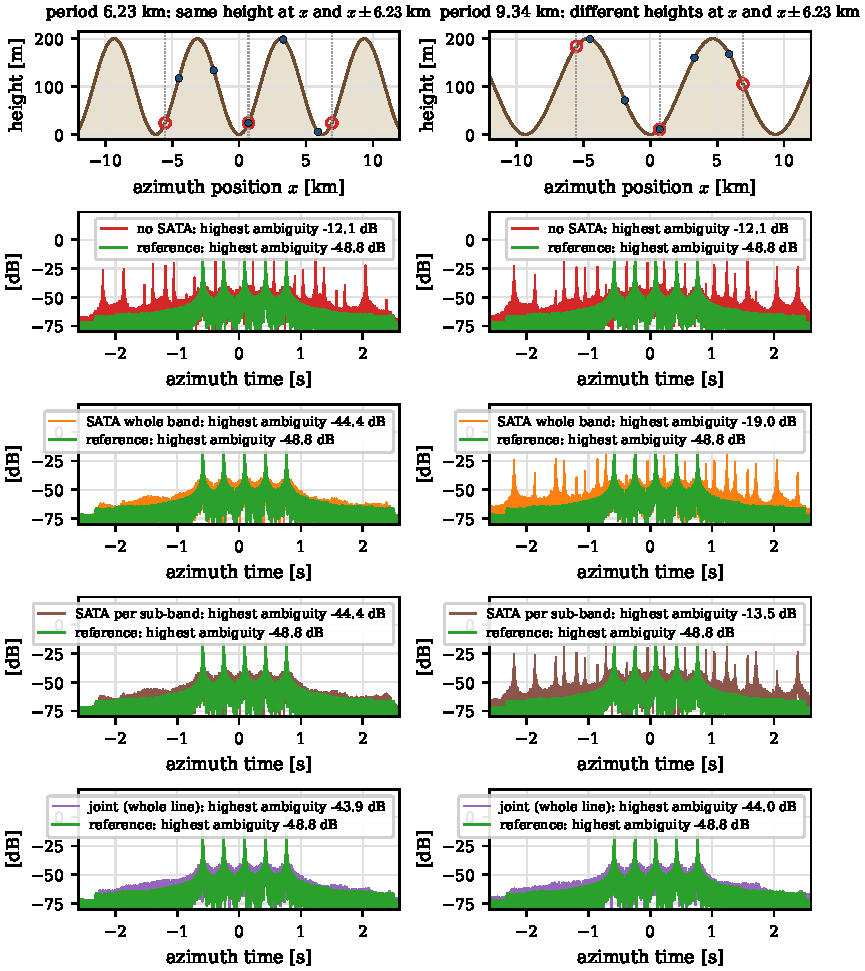
\includegraphics[width=\linewidth]{figures/sata_controls.pdf}
\caption[SATA on terrains with and without the period of the folds]{Five targets on $h=100-100\cos(2\pi x/P)$, four channels,
$\bxt=[0,100,39.9,33.5]$\,\si{m}. Left: $P=X=\SI{6.23}{km}$; right: $P=1.5X$. Top: terrain, targets, and the three positions
$x$, $x\pm X$ folded onto the same channel bin for the middle target (red circles). Below: azimuth impulse responses of the
reference and, from top to bottom, of no SATA, SATA whole band, SATA per sub-band and the joint reconstruction over the whole line.
Every method reads only the DEM.}
\label{fig:satacontrols}
\end{figure}

The residual left by SATA is not an implementation detail. Writing the leakage matrix $\mathbf L$ of
\cref{sec:sata-limit} with the heights of the DEM at the folded positions predicts the level it leaves without any simulation;
over the \PredRuns{} runs of the audit (\cref{sec:audit}) the prediction agrees with the simulation within \SI{\PredRmsWhole}{dB}
rms for SATA whole band and \SI{\PredRmsSub}{dB} rms per sub-band (\cref{fig:sataprediction}).

\begin{figure}[htbp]
\centering
\begin{tikzpicture}
\begin{groupplot}[group style={group size=2 by 1, horizontal sep=1.5cm},
  width=0.46\linewidth, height=0.46\linewidth, xmin=-70, xmax=5, ymin=-70, ymax=5,
  xlabel={predicted from the DEM [dB]}, grid=major, grid style={gray!20},
  scatter/classes={2={mark=*,cnone,mark size=0.8pt}, 3={mark=*,cwhole,mark size=0.8pt}, 4={mark=*,cjoint,mark size=0.8pt},
                   6={mark=*,cocc,mark size=0.8pt}, 8={mark=*,cref,mark size=0.8pt}},
  legend style={font=\scriptsize,draw=none,fill=white,fill opacity=0.85,text opacity=1}, legend pos=north west]
\nextgroupplot[ylabel={simulated [dB]}, title={\small SATA whole band}]
  \addplot[scatter,only marks,scatter src=explicit symbolic,opacity=0.6] table[x=pwhole,y=swhole,meta=nrx] {data/sata_prediction.dat};
  \addplot[gray,dashed,domain=-70:5] {x};
  \legend{$\Nrx=2$,3,4,6,8}
\nextgroupplot[title={\small SATA per sub-band}]
  \addplot[scatter,only marks,scatter src=explicit symbolic,opacity=0.6] table[x=psub,y=ssub,meta=nrx] {data/sata_prediction.dat};
  \addplot[gray,dashed,domain=-70:5] {x};
\end{groupplot}
\end{tikzpicture}
\caption[Prediction of the level left by SATA]{Highest ambiguity left by SATA, predicted only from the geometry and the DEM
(the leakage of the folded parcels) against the simulation, for the \PredRuns{} runs of the audit, coloured by the number of channels.}
\label{fig:sataprediction}
\end{figure}

The extreme case is a single target at the height of the reference point on a gently varying terrain
(\cref{fig:satarefpoint}): without correction there is nothing to correct (\SI{-63.7}{dB}), but SATA gives every bin the phase of
the terrain at the labelled position, and the energy of the target receives the phase of other places: \SI{-36.3}{dB} whole band and
\SI{-27.8}{dB} per sub-band. The joint reconstruction leaves the target untouched (\SI{-63.5}{dB}).

\begin{figure}[htbp]
\centering
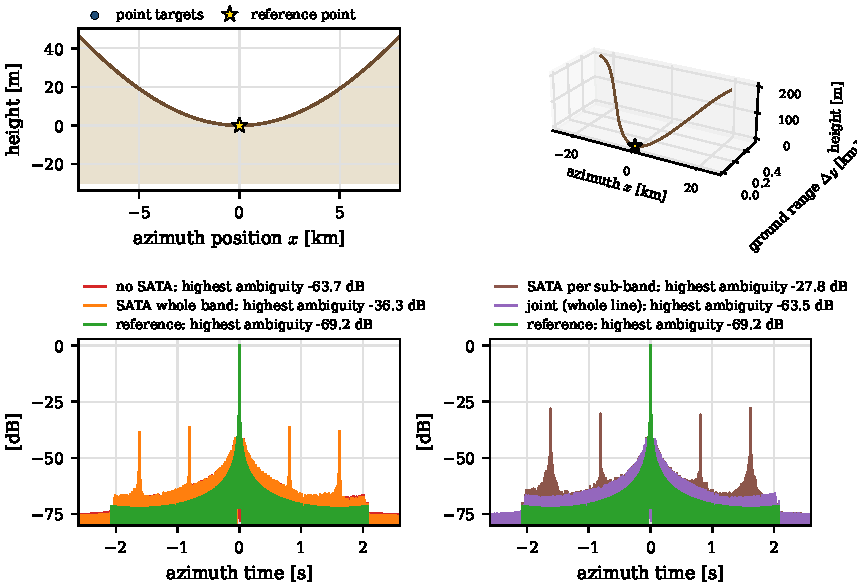
\includegraphics[width=\linewidth]{figures/sata_refpoint.pdf}
\caption[SATA can degrade a target at the reference height]{One target at the reference point ($x=0$, $h=0$) on the terrain
$h=100-100\cos(2\pi x/\SI{50}{km})$, four channels, $\bxt=[0,100,39.9,33.5]$\,\si{m}. Top: the terrain near the target (left) and
along the whole azimuth line (right). Bottom: impulse responses; every method reads only the DEM.}
\label{fig:satarefpoint}
\end{figure}

\subsection{Correction maps that use the target positions}\label{sec:sata-maps}

During the project, maps were also built from the simulated targets: the $\dC$ of each target written at its cell and
copied at the folded positions $\pm X$ (\emph{block map with copies}), or the value of the nearest target. With such maps
SATA per channel reaches the oracle for isolated targets, because the map then encodes exactly which parcel is occupied.
A real scene provides no such information. These maps are kept in the code for reference but are \emph{not} part of any
method evaluated in \cref{ch:results}; every method there receives only the system parameters and the DEM, and removing the
target list from the configuration given to the methods does not change a single bit of their output.
